
\newcommand{\insertDatasetLanguageComparison}{
\begin{figure}%
  \centering
  % \subfloat[\centering Speech-text paired datasets]{
  \begin{subfigure}[t]{0.5\linewidth}
    \centering
    \resizebox{\linewidth}{!}{

    \begin{tikzpicture}

      \begin{axis}[
      % yticklabel style={
      %         /pgf/number format/relative*=5,
      %       },
          width=\linewidth,
          enlargelimits=0.2,
          xmode=log,
          ymode=log,
          xlabel={\# languages},
          ylabel={\# hours},
          xmin=5, xmax=4500,
          ymin=1000, ymax=450000,
          ytick={1000, 10000, 100000,1000000},
          yticklabels = {$10^3$, $10^4$, $10^5$, $10^6$},
          legend pos=north west,
          ymajorgrids=true,
          grid style=dashed,
          log ticks with fixed point,
          % every node near coord/.append style={font=\small}
        ]
        \addplot[
          scatter, only marks,
          scatter/classes={
              a={mark = o, black},
              c={mark = o, black},
              b={mark = *, metablue}
            },
          point meta=explicit symbolic,
          visualization depends on={value \thisrow{z} \as \Label},
          visualization depends on={\thisrow{yshift} \as \yShift},
          visualization depends on={\thisrow{xshift} \as \xShift},
          nodes near coords*={\Label},
          nodes near coords style={   
                yshift=\yShift,
                xshift=\xShift,
         },
        ]
        table[row sep=\\,col sep=&,meta=class]{
            x    &   y    & class & z & xshift & yshift\\
            8  &   49400   &  a & MLS  & 0  & 0\\
            25 &1400 & c & BABEL  & 16 & 0 \\
            16 & 1800 & a & VoxPopuli  & -7 & 2 \\
            98 &17127& a & CommonVoice  & 0 & 0\\
            102 &1200 & a & FLEURS  & 4 & -13\\
            8 &999 & a & M-AILABS  & -4 & -13\\
            % 107 &6200& a & VoxLingua \\
            % 40 & 17000 & a & Dhwani \\
            699 & 13725 & a & CMU Wilderness  & 0 & -14 \\
            1107 & 44700& b & {\MMS}  & 0 & 0\\
            % 3900 & 6500 & b & GRN \\
          };
      \end{axis}
   \end{tikzpicture}
}
\label{fig:lab-speech-datasets}
\caption{Labeled Datasets.}
\end{subfigure}\hfill 
  \begin{subfigure}[t]{0.5\linewidth}
  \centering
    \resizebox{\linewidth}{!}{
    \begin{tikzpicture}
      \begin{axis}[
          width=\linewidth,
          enlargelimits=0.2,
          xmode=log,
          ymode=log,
          xlabel={\# languages},
          ylabel={\# hours},
          xmin=5, xmax=4500,
          ymin=1000, ymax=450000,
          ytick={1000, 10000, 100000,1000000},
          yticklabels = {$10^3$, $10^4$, $10^5$, $10^6$},
          legend pos=north west,
          ymajorgrids=true,
          grid style=dashed,
          log ticks with fixed point,
          % every tick label/.append style={font=\large}
        ]
        \addplot[
          scatter, only marks,
          scatter/classes={
              a={mark = o, black},
              b={mark = *, metablue}
            },
          point meta=explicit symbolic,
          visualization depends on={value \thisrow{z} \as \Label},
          visualization depends on={\thisrow{yshift} \as \yShift},
          visualization depends on={\thisrow{xshift} \as \xShift},
          nodes near coords*={\Label},
          nodes near coords style={   
                yshift=\yShift,
                xshift=\xShift,
         },
        ]
        table[row sep=\\,col sep=&,meta=class]{
            x    &   y    & class & z  & xshift & yshift\\
            23 & 400000& a & VoxPopuli &0 & 0\\
            107 & 6200 & a & VoxLingua107 &0 & -15 \\
            40 & 17000 & a & Dhwani &0  & 0 \\
            3809 & 7700 & b & \GRN & -3 & 0 \\
            1362 & 55000 & b & \MMSU & -3 & 0 \\
          };
      \end{axis}
    \end{tikzpicture}
    
  }
  \label{fig:unlab-speech-datasets}
  \caption{Unlabeled Datasets.}
  \end{subfigure}
\caption{
\textbf{Dataset Overview.}
\MMS{}, \MMSU{} and \GRN{} compared to existing multilingual speech corpora in terms of the supported languages and dataset size. 
We compare to BABEL~\citep{gales2014babel}, CMU Wilderness~\citep{black2019cmu}, CommonVoice~\citep{ardila2019common}, Dhwani~\citep{javed2022towards}, FLEURS~\citep{conneau2022fleurs}, M-AILABS~\citep{mailabs}, MLS~\citep{pratap2020mls}, VoxLingua107~\citep{valk2020voxlingua}, and VoxPopuli~\citep{wang2021voxpopuli} .
}
\label{fig:datasets-comp}
% \end{subfigure}
\end{figure}
}


\newcommand{\insertGenderAnalysis}{
\definecolor{metagray}{RGB}{28,43,51}
\definecolor{metablue}{RGB}{0,75,185}
\definecolor{metadarkblue}{RGB}{0,30,110}
\begin{figure}
\centering
% \resizebox{.95\linewidth}{!}{%
\begin{tikzpicture}
\begin{axis}[
ybar,
bar width=.15in,
% bar shift=50,
width=.55*\textwidth,
height=.4\textwidth,
legend style={at={(0.95,0.98)},draw=none},
legend cell align={left},
legend columns=2,
nodes near coords align={vertical},
ylabel={CER},
ymin=0,
ymax=15,
symbolic x coords={Overall,Female,Male},
enlarge x limits=0.3,
xtick=data]
\addplot[fill=metablue] coordinates {
(Overall,12.37)
(Female,12.44)
(Male,12.26)
};
\addplot[fill=metagray, pattern= north east lines] coordinates {
(Overall,6.35)
(Female,6.49)
(Male,6.24)
};
\legend{\modelname{} data, FLEURS data}
\end{axis}
\end{tikzpicture}
\caption{
\textbf{Analysis of Gender Bias.}
We compare the character error rate (CER) of automatic speech recognition models trained on \MMS{} data and FLEURS data for male and female spakers.
Results are on the development sets of 27 languages of the FLEURS benchmark for which \MMS{} provides data and for which there are at least 50 samples for each gender.
}
\label{fig:rai-gender-analysis}
\end{figure}
}


\newcommand{\insertGRNHours}{
\begin{figure}[t]
  \centering
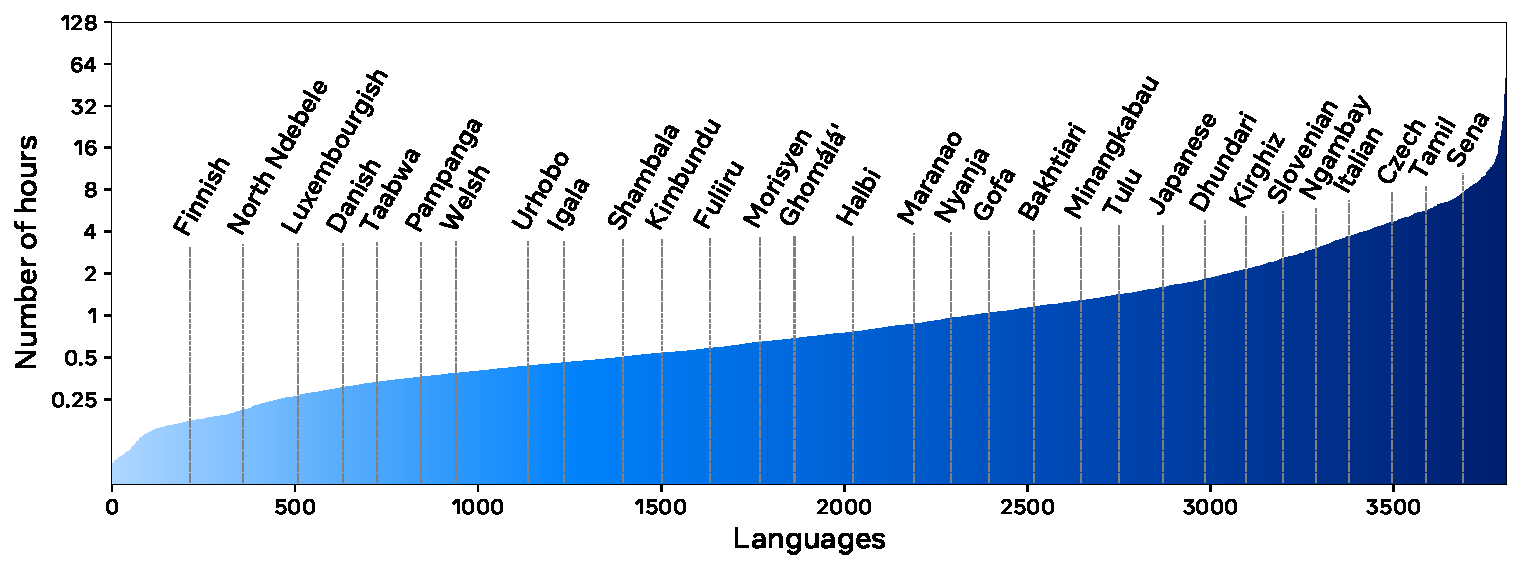
\includegraphics[width=\linewidth]{images/mmsunlab.pdf}
\caption{
\textbf{\GRN{}: Amount of Speech Data across Languages.}
We show the size of the training data sets and name a few of the \numgrnlang{} languages.
} 
\label{fig:data-grnhrs}
\end{figure}
}

\newcommand{\insertMMSHours}{
\begin{figure}[t]
  \centering
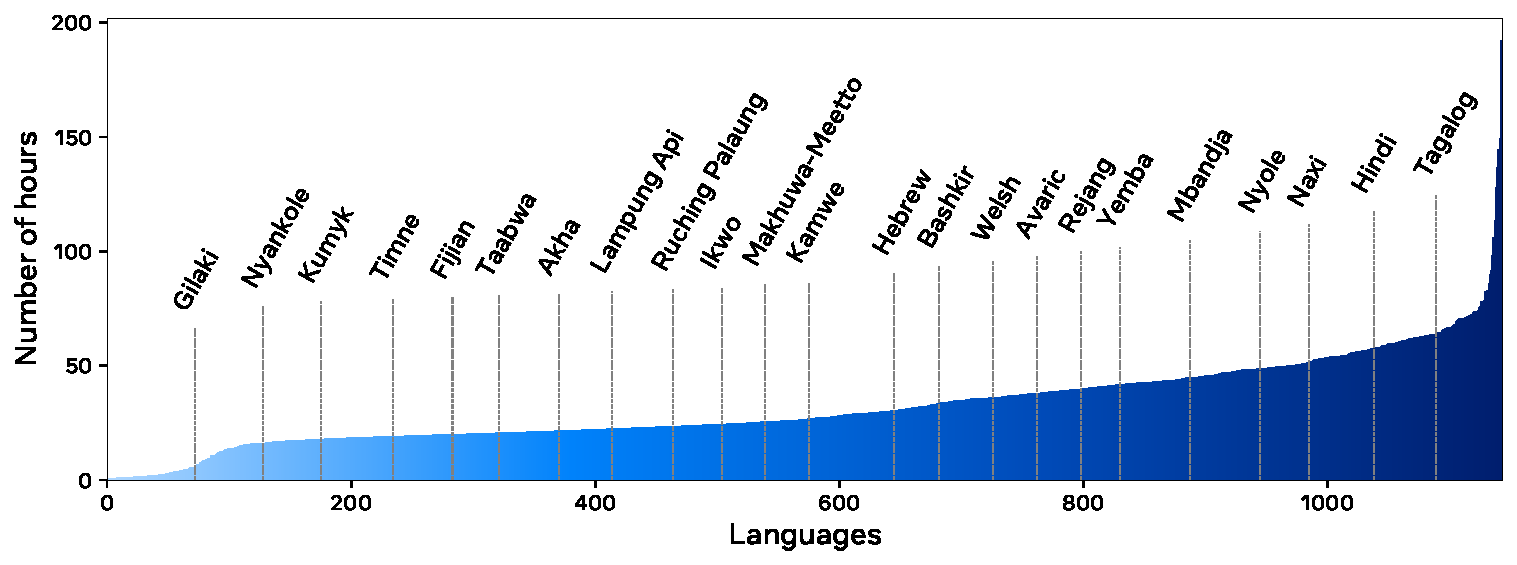
\includegraphics[width=\linewidth]{images/mmslab.pdf}
\caption{
\textbf{\MMS{}: Amount of Speech Data across Languages.}
We show the size of the training data sets and name some of the \nummmslang{} languages.
}
\label{fig:data-mmshrs}
\end{figure}
}


\newcommand{\insertPretrainSetup}{
\begin{table*}[t]
\begin{center}
% \scriptsize
\resizebox{1\linewidth}{!}{
\begin{tabular}[b]{lrlrrrrrrr}
\toprule
Model & \#langs & Datasets & $B$ & $M$ & $F$ & $A$ & \#params \\
\midrule
\textit{Prior work} \\
XLSR-53 & 53 & MLS, CV, BBL & 24 & 1024 & 4096 & 16 & 317M \\
VP-100K & 23 & VP-100K & 24 & 1024 & 4096 & 16 & 317M \\
XLS-R (0.3B) & 128 & VP-400K, MLS, CV, VL, BBL & 24 & 1024 & 4096 & 16 & 317M \\
XLS-R (1B)   & 128 & VP-400K, MLS, CV, VL, BBL & 48 & 1024 & 4096 & 16 & 965M \\
\midrule
\modelnameb{0.3} & \numptlang{} & \MMS{}, FL, VP-400K, MLS, CV, VL, BBL & 24 & 1024 & 4096 & 16 & 317M \\
\modelnameb{1} & \numptlang{} & \MMS{}, FL, VP-400K, MLS, CV, VL, BBL & 48 & 1024 & 4096 & 16 & 965M \\
\bottomrule
\end{tabular}
}
\caption{\textbf{Self-supervised Models.}
Details of our models including prior work: XLSR-53~\citep{conneau2020unsupervised}, VP-100K~\citep{wang2021voxpopuli}, XLS-R~\citep{babu22_interspeech} and the \modelname{} models: 
the number of languages (\#langs), pretraining data (Datasets), the number of Transformer blocks ($B$), the number of hidden states ($M$), the inner dimension of feed-forward blocks ($F$), the number of attention heads ($A$) and the total number of parameters (\#params).
\label{tab:pretrain-models}}
\end{center}
\vspace{-0.4cm}
\end{table*}
}




\newcommand{\insertPretrainComparisonASR}{
\begin{figure}
\centering
  % \resizebox{.95\linewidth}{!}{%
\begin{tikzpicture}
\begin{axis}[
    ybar,
    bar width=.25in,
    % bar shift=50,
    width=.5*\textwidth,
    height=.35\textwidth,
    legend style={at={(0.95,0.95)},draw=none},
    nodes near coords align={vertical},
    ylabel={CER},
    ymin=12, 
    ymax=18,
    symbolic x coords={300M, 1B, 2B},
    enlarge x limits=0.4,
    xtick=data]
    \addplot[fill=metagray, pattern= north east lines] coordinates {
        (300M, 16.96)
        (1B, 13.92)
    };
    \addplot[fill=metablue] coordinates {
        (300M, 16.40)
        (1B, 13.20) 
    };
    
    \legend{XLS-R, \modelname{}}
\end{axis}
\end{tikzpicture}
% }
\caption{\textbf{\modelname{} vs. XLS-R.} 
Character error rate (CER) on 61 FLEURS languages when fine-tuning multilingual ASR models on \MMS{} data. 
We report average performance on FLEURS dev data. 
}
\label{fig:pretrain-comparison-asr}
\end{figure}
}


\newcommand{\insertResultsASRCapacity}{
\begin{figure}
\centering
  % \resizebox{.95\linewidth}{!}{%
\begin{tikzpicture}
\begin{axis}[
    ybar,
    bar width=.25in,
    % bar shift=50,
    width=.6*\textwidth,
    height=.35\textwidth,
    legend style={at={(0.95,0.95)}},
    nodes near coords align={vertical},
    ylabel={CER},
    ymin=10,
    symbolic x coords={300M, 1B, 2B},
    enlarge x limits=0.2,
    xtick=data,
    legend cell align={left}
    ]
    \addplot[fill=metablue] coordinates {
        (300M, 18.07)
        (1B, 15.17)
        (2B, 13.49)
    };
    \addplot[fill=black] coordinates {
        (300M, 14.23)
        (1B, 12.05)
        (2B, 0)
    };    
    \legend{FLEURS, CV}
    
\end{axis}
\end{tikzpicture}
% }
\caption{\textbf{Increasing model capacity for multilingual ASR.} 
We fine-tune multilinugal ASR models on 61 languages of the \MMS{} data and report average character error rate on the dev sets of 61 FLEURS languages, CV (\ma{XX}) languages for different model sizes without language models.}
\label{fig:results_asr_capacity}
\end{figure}
}


\newcommand{\insertResultsASRLangScaling}{
\begin{center}
\begin{figure}[t]
\centering
\begin{tikzpicture}
\begin{axis}[
width=0.7\columnwidth,
height=.4\columnwidth,
legend style={font=\small,%fill=none,
at={(1.0,0.65)},
anchor=east,legend columns=1,draw=none,legend columns=2},
legend cell align={left},
% xticklabels from table={\visionEfficiencyTableTrainingTime}{hours},
% xticklabel style={text height=1.5ex},
% xticklabel style={font=\small},
% xtick=data,
% yticklabel style={font=\small},
xtick={61,128,256,512,1107},
x tick label style={xshift={(\ticknum==0)*-0.6em}},
x tick label style={xshift={(\ticknum==1)*0.2em}},
x tick label style={xshift={(\ticknum==2)*0.1em}},
% xticklabels={$5$,$10$,$15$,$20$,$25$,$30$,$35$,$40$},
% nodes near coords,
% nodes near coords align={vertical},
% ymin=10,ymax=22,
% xmin=0,xmax=50,
% bar width=2pt,
ylabel={Character Error Rate},
ylabel near ticks, %ylabel shift={-10pt}
% ylabel style={font=\small},
xlabel={Number of Languages supported by Model},
xlabel near ticks,
% log basis x={2},
% xmode=log,
% xlabel style={font=\small},
% grid=both,
% style=thick,
% xticklabel={$\pgfmathprintnumber{\tick}\%$},
% nodes near coords={\pgfmathprintnumber\pgfplotspointmeta\%}
]
\addplot[blue,dashed,line width=1,,mark=+,mark options={scale=1}] coordinates {
    (61, 15.46)
    (128, 18.84)
    (256, 20.63)
    (512, 19.93)
    (1107, 20.69)
};
\addplot[metablue,line width=1,mark=+,mark options={scale=1}] coordinates {
    (61, 13.2)
    (128, 13.29)
    (256, 13.74)
    (512, 13.57)
    (1107, 13.63)
};
\addplot[black,dashdotted,line width=1,mark=+,mark options={scale=1}] coordinates {
    (61, 9.0)
    (128, 9.44)
    (256, 10.44)
    (512, 10.45)
    (1107, 11.07)
};
\addplot[metagray,loosely dashdotted,line width=1,mark=+,mark options={scale=1}] coordinates {
    (61, 7.47)
    (128, 7.34)
    (256, 7.72)
    (512, 7.7)
    (1107, 7.63)
};
\legend{FLEURS-61 (Dense), FLEURS-61 (LSAH), CV-49 (Dense), CV-49 (LSAH)}
\end{axis}
\end{tikzpicture}
\caption{
\textbf{Scaling Multilingual ASR to \nummmslang{} Languages.}
We fine-tune both dense and LSAH models with 61, 128, 256, 512 and \nummmslang{} languages on \MMS{} data and show average CER on 61 languages of FLEURS and 49 languages of CommonVoice. 
LSAH models have language-specific adapter modules and output layers.
}
\label{fig:results_asr_scale_lang}
\end{figure}
\end{center}
}

\newcommand{\insertResultsLIDFLVLCompare}{
\begin{figure}
\centering
\begin{tikzpicture}
\begin{axis}[
    ybar,
    bar width=.12in,
    % bar shift=50,
    width=0.9\linewidth,
    height=2in,
    legend style={fill=none, at={(0.96,0.92)},draw=none},
    nodes near coords align={vertical},
    scaled y ticks = false,
    legend columns=1,
    ylabel={Dev Accuracy},
    xlabel={Evaluation Set},
    ymin=70,
    xmax=3.5,
    xtick={1, 2},
    legend cell align={left},
    xticklabels={FLEURS, VoxLingua-107},
    enlarge x limits=0.2,
    % x tick label style={rotate=45}, 
    xtick=data]
    \addlegendimage{empty legend}
   \addlegendentry[yshift=10pt]{Model Trained on}
    \addplot[fill=lightgray, pattern=] coordinates {
        % FLEURS
        (1, 98.46)
        (2, 91.51)
    };	
    \addlegendentry{FLEURS}
    \addplot[fill=metagray] coordinates {
        % VL
        (1, 98.09)
        (2, 99.05)
    };
    \addlegendentry{VoxLingua-107}
    \addplot[fill=metablue, pattern=dots] coordinates {
        % MMS
        (1, 91.58)
        (2, 88.43)
    };
    \addlegendentry{\MMSU{}}
    \addplot[fill=metablue, pattern=north east lines] coordinates {
        % GRN
       (1,  92.01)
       (2, 84.23)
    };
    \addlegendentry{\GRN{}}
    \addplot[fill=metablue] coordinates {
        % MMS + GRN
       (1, 95.94)
       (2, 89.92)
    };
    \addlegendentry{\MMSUboth{}}
    \addplot[black,sharp plot,dashed] coordinates {(0.85,98.09) (1.33,98.09)};
    \addplot[black,<->,sharp plot,dashed] coordinates {(1.26,98.09)(1.26,95.94)};
    \node[font=\scriptsize] at (axis cs: 1.41,97) {-2.1\%};
    \addplot[black,sharp plot,dashed] coordinates {(1.7,91.51) (2.33,91.51)};
    \addplot[black,<->,sharp plot,dashed] coordinates {(2.26,91.51)(2.26,89.92)};
    \node[font=\scriptsize] at (axis cs: 2.43,90.8) {-1.6\%};    
    % \addplot[red,sharp plot,update limits=false] coordinates { (1,98) (2,98) };
    % \coordinate (A) at (0.755, 85 );
    % \coordinate (B) at (1.955, 85);
\end{axis}
% \node[rotate=90, color=black] at (A) {in-domain};
% \node[rotate=90, color=white] at (B) {in-domain};
\end{tikzpicture}
% }
\caption{
\textbf{LID Performance with Different Training Datasets.} 
Models trained on \MMSUboth{} are very competitive to models trained on existing data (FLEURS, VoxLingua-107) when evaluated out-of-domain (comparison in dashed line).
We train models on data from \MMSU{}, \GRN{}, FLEURS and VoxLingua-107 on a common subset of 72 languages and evaluate on FLEURS and VoxLingua-107.
}
\label{fig:lid-fl-vl-comp2}
\end{figure}
}




\newcommand{\insertLIDResultsScaling}{
\begin{table*}[t]
\begin{small}
\centering
\begin{tabular}{lrrrrrr}
\toprule
& \#lang & \multicolumn{2}{c}{in-domain} & \multicolumn{2}{c}{out-of-domain}\\
\cmidrule(lr){3-4}\cmidrule(lr){5-6}
 &  &  FLEURS & VL &  BABEL & VoxPopuli  \\ 
&  &   (102 lang.) &  (33 lang.) & (23 lang.) & (25 lang.) \\ 
\midrule
\multicolumn{2}{l}{\textit{Prior Work}} \\
mSLAM~\citep{Bapna2022mSLAMMM} & 102 & 77.7 & - & - & -  \\
Whisper~\citep{radford2022whisper}  & 82 & 64.5 & - & - & -  \\
ASRL~\citep{chen2023improving} & 102 & 95.9 & - & - & -  \\
XLS-R~\citep{babu22_interspeech}  & 107 & - & 94.3 & - & -  \\
SpeechBrain~\citep{speechbrain}  & 107 & - & 93.3 & - & -  \\
AmberNet~\citep{jia2022ambernet}  & 107 & - & 95.3 & - & -  \\
% CL~\cite{speechbrain}  & 45 & - & - & 84.9 & - & - \\
\midrule
\multicolumn{2}{l}{\textit{Our Baselines (based on existing datasets)}} \\
\modelname{} (FL) & 102 & 96.2 & - & - & - \\
\modelname{} (VL) & 107 & - & 94.7 & - & - \\
\modelname{} (FL + VL) & 126 & 97.4 & 94.3 & 78 &	87.8 \\
% CL  & 45 &x & x & & x & x \\
\midrule
\multicolumn{2}{l}{\textit{This Work}} \\
\modelname{} (\MMSUboth{}+FL+VL) & 126 & 97.5 &	93.9 & 84.1  & 87.3 \\
& 256 & 97.2 &	93.4 & 80.1 & 87.6 \\
& 512 & 96.8 &	92.9 & 81.6 & 85.6\\
& 1,024 & 97 & 92.8 & 80.5 & 86.2 \\
& 2,048 & 97.3 & 92.8 & 81.5 & 86.6 \\
&  \numlidlang{} & 97.2  & 93.9	 & 80.5&  87.1   \\
\bottomrule
\end{tabular}
\caption{
\textbf{Scaling LID to \numlidlang{} Languages.}
We show test accuracy of LID models trained on an increasing number of languages using data from FLEURS (FL), VoxLingua-107 (VL) and \MMSUboth{}; smaller language subsets are included in the larger subsets. 
There is little performance degradation when scaling to more languages.
We also show results from the literature as well as baselines trained only on FL or VL.} 
\label{tab:lid-scale}
\end{small}
\end{table*}
}

\newcommand{\insertDataRAIWords}{

\pgfplotstableread[row sep=\\,col sep=&]{
lang & mmstr & cctr & mmsout & flout \\
amh & 12.48 & 3.86 & 5.42 & 3.93\\
ara & 12.29 & 3.89 & 4.23 & 3.62\\
asm & 21.93 & 4.25 & 5.76 & 4.53\\
azj & 13.41 & 3.13 & 4.08 & 3.80\\
ben & 22.76 & 3.92 & 8.56 & 7.98\\
bul & 13.04 & 3.78 & 4.26 & 4.04\\
cat & 12.69 & 3.57 & 4.36 & 4.06\\
ceb & 19.23 & 5.94 & 6.69 & 6.32\\
cym & 16.32 & 4.51 & 5.60 & 4.81\\
deu & 22.40 & 3.50 & 8.37 & 8.18\\
ell & 15.32 & 3.59 & 5.60 & 3.41\\
eng & 20.31 & 5.17 & 6.93 & 6.66\\
fas & 21.52 & 6.14 & 9.25 & 6.78\\
fin & 16.25 & 3.57 & 4.65 & 4.60\\
fra & 15.27 & 4.75 & 3.96 & 3.44\\
guj & 18.38 & 4.33 & 4.79 & 4.11\\
hau & 25.44 & 7.78 & 10.63 & 7.81\\
heb & 13.67 & 3.64 & 4.25 & 3.72\\
hin & 15.35 & 3.62 & 4.23 & 3.43\\
hun & 19.45 & 3.63 & 6.63 & 6.65\\
ind & 23.56 & 6.15 & 6.35 & 6.28\\
jav & 29.96 & 5.61 & 9.23 & 8.88\\
kan & 12.66 & 2.90 & 4.84 & 4.29\\
kaz & 13.27 & 3.86 & 5.84 & 5.32\\
kir & 12.48 & 4.01 & 3.82 & 3.39\\
kor & 9.94 & 2.31 & 3.12 & 2.55\\
lav & 20.52 & 4.95 & 6.47 & 6.21\\
mar & 18.40 & 4.04 & 5.71 & 4.95\\
mon & 18.50 & 2.97 & 5.61 & 3.63\\
nld & 13.95 & 2.85 & 4.45 & 4.00\\
nya & 18.12 & 5.27 & 5.63 & 5.03\\
ory & 21.16 & 4.50 & 8.13 & 6.95\\
pan & 26.67 & 6.58 & 8.49 & 6.93\\
pol & 10.49 & 2.71 & 3.18 & 2.87\\
ron & 19.95 & 5.48 & 7.59 & 7.05\\
rus & 18.48 & 3.90 & 7.71 & 7.70\\
sna & 14.13 & 3.32 & 4.10 & 3.21\\
som & 16.89 & 3.75 & 6.44 & 5.46\\
spa & 10.07 & 2.08 & 2.38 & 2.13\\
swe & 16.22 & 3.97 & 5.26 & 4.43\\
swh & 13.87 & 3.81 & 3.75 & 3.70\\
tam & 9.21 & 2.08 & 3.64 & 3.33\\
tel & 8.79 & 2.20 & 4.18 & 3.15\\
tgk & 22.20 & 6.79 & 8.64 & 8.35\\
tgl & 10.76 & 3.00 & 2.67 & 2.57\\
tur & 8.79 & 2.18 & 2.98 & 2.25\\
ukr & 18.04 & 4.57 & 7.13 & 6.40\\
urd & 19.99 & 6.96 & 7.70 & 6.42\\
vie & 31.22 & 6.88 & 7.12 & 6.21\\
yor & 34.67 & 9.22 & 16.32 & 14.72\\
zlm & 24.54 & 6.06 & 7.26 & 6.68\\
}\dataRAIWords 
\begin{figure}
\centering
  % \resizebox{.95\linewidth}{!}{%
\begin{tikzpicture}
\begin{axis}[
width=1*\textwidth,
height=.4\textwidth,
ylabel={Cumulative Relative Frequency (\%)},
ylabel style={align=center,text width=5cm},
legend style={%font=\small,
at={(0.88,0.87)},
anchor=east,legend columns=4,draw=none},
xticklabels from table={\dataRAIWords}{lang},
x tick label style={rotate=45,anchor=east,font=\tiny},
enlarge x limits=0,
xtick=data]
\addplot[dashed,black,mark=square*,mark options={solid,scale=0.5,fill=black}] table[xticklabels from table={\dataRAIWords}{lang},x expr=\coordindex,x=lang,y=mmstr]{\dataRAIWords};
\addplot[solid,metablue,mark=diamond*,mark options={solid,scale=0.5,fill=metablue}] table[xticklabels from table={\dataRAIWords}{lang},x expr=\coordindex,x=lang,y=mmsout]{\dataRAIWords};
\addplot[dashdotdotted,red,mark=otimes,mark options={solid,scale=0.5,fill=red}] table[xticklabels from table={\dataRAIWords}{lang},x expr=\coordindex,x=lang,y=flout]{\dataRAIWords};
\legend{\MMS{} train, \MMS{} ASR output, FLEURS ASR output}
\end{axis}
\end{tikzpicture}
% }
\caption{
\textbf{Analysis of Language Produced by \modelname{} ASR Models.}
\modelname{} models generate biased words at a slightly increased rate of 0.7\% absolute compared to models trained on FLEURS data.
We focus on words that occur at least twice as often in the \MMS{} training data compared to Common Crawl (in terms of relative frequency).
We compare the cumulative relative frequency of these words in the \modelname{} model output and the output of ASR models trained on FLEURS data.
ASR outputs are based on transcribing the development sets of 51 languages.
}
\label{fig:data-rai-words}
\end{figure}
}


\newcommand{\insertComparisonWithOtherDatasets}{
\begin{figure}
\centering
\begin{minipage}[t]{0.4\textwidth}
\begin{tikzpicture}
\begin{axis}[
    ybar,
    enlargelimits=0.1,
    bar width=.08in,
    % bar shift=50,
    width=\textwidth,
    height=2in,
    legend style={at={(0.83,0.95)},draw=none},
    legend cell align={left},
    % legend columns=-1,
    nodes near coords align={vertical},
    ylabel={CER},
    ymin=5,
    symbolic x coords={eng, por, tel},
    legend style={fill=none, nodes={scale=0.9, transform shape}}, 
    x tick label style={rotate=45,font=\scriptsize}, 
    enlarge x limits=0.15,
    xtick=data]
    \addplot[fill=black, pattern=north east lines] coordinates {
        (eng, 17.16)
        (por, 10.49)
        (tel, 18.71)
    };
    \addplot[fill=metablue] coordinates {
        (eng, 12.44)
        (por, 8.256)
        (tel, 16.60)
    };    
    \legend{CMU Wilderness, {\MMS}}
\end{axis}
\end{tikzpicture}
% }
\caption{
\textbf{{\MMS} vs. CMU Wilderness.} 
Character Error Rate of ASR models in English (eng), Portuguese (por) and Telugu (tel) on the FLEURS dev set.
}
\label{fig:data-compare-cmu}
\end{minipage}\hfill
\begin{minipage}[t]{0.55\textwidth}
\begin{tikzpicture}
\begin{axis}[
    % ybar,
    % bar width=.03in,
    % bar shift=50,
    width=1.05\linewidth,
    height=2in,
    legend style={fill=none, at={(0.67,0.97)}, draw=none},
    legend cell align={left},
    nodes near coords align={vertical},
    scaled y ticks = false,
    % legend columns=-1,
    ylabel={CER},
    ymin=0,
    symbolic x coords={spa,cat,pol,deu,por,rus,ukr,tur,swh,fra,nld,fas,eng,cym,lug,ara,tam,tha},
    enlarge x limits=0.04,
    x tick label style={rotate=45,font=\scriptsize}, 
    xtick=data]
    % \addplot[fill=black, pattern=north east lines] coordinates {
     \addplot[black,line width=0.6,mark=square*,mark options={scale=0.5}, dashed] coordinates {
(spa, 4.891304347826087)
(cat, 5.725425074907043)
(pol, 5.801607040367323)
(deu, 5.9194078623594955)
(por, 6.664313863890359)
(rus, 7.034013011395887)
(ukr, 7.865942118075193)
(tur, 7.907471931862176)
(swh, 7.922350472193075)
(fra, 8.30560720227028)
(nld, 9.047417442845047)
(fas, 9.172106615134448)
(eng, 9.468897855518914)
(cym, 12.19765442816048)
(lug, 12.924718556148367)
(ara, 15.041513805754006)
(tam, 15.646954117669337)
(tha, 16.505637617410347)
    };				
    % \addplot[fill=metablue] coordinates {
    \addplot[metablue,line width=0.6,mark=*,mark options={solid, scale=0.5}] coordinates {
(spa, 6.516737796745799)
(cat, 7.880581928450236)
(pol, 7.891716089535106)
(deu, 9.09466721785862)
(por, 8.164225633786248)
(rus, 9.717067633061172)
(ukr, 11.485406575032581)
(tur, 9.388308168795973)
(swh, 11.60620596612202)
(fra, 11.689010666405714)
(nld, 12.320067739204065)
(fas, 13.180779110597884)
(eng, 13.477254572639945)
(cym, 17.19859061430833)
(lug, 15.717458453526664)
(ara, 14.771191349681406)
(tam, 17.91171959325115)
(tha, 22.498607402854343)

    };
    \legend{Common Voice, \MMS{}}
\end{axis}
\end{tikzpicture}
% }
\caption{\textbf{{\MMS} vs. Common Voice.}
Character Error Rate on FLEURS dev set for ASR models trained on Common Voice (CV) data and {\MMS} data for 18 languages. }
\label{fig:compare-cv}
\end{minipage}

\end{figure}
}

\newcommand{\insertUromanXsampaExamples}{
\begin{table}
\centering
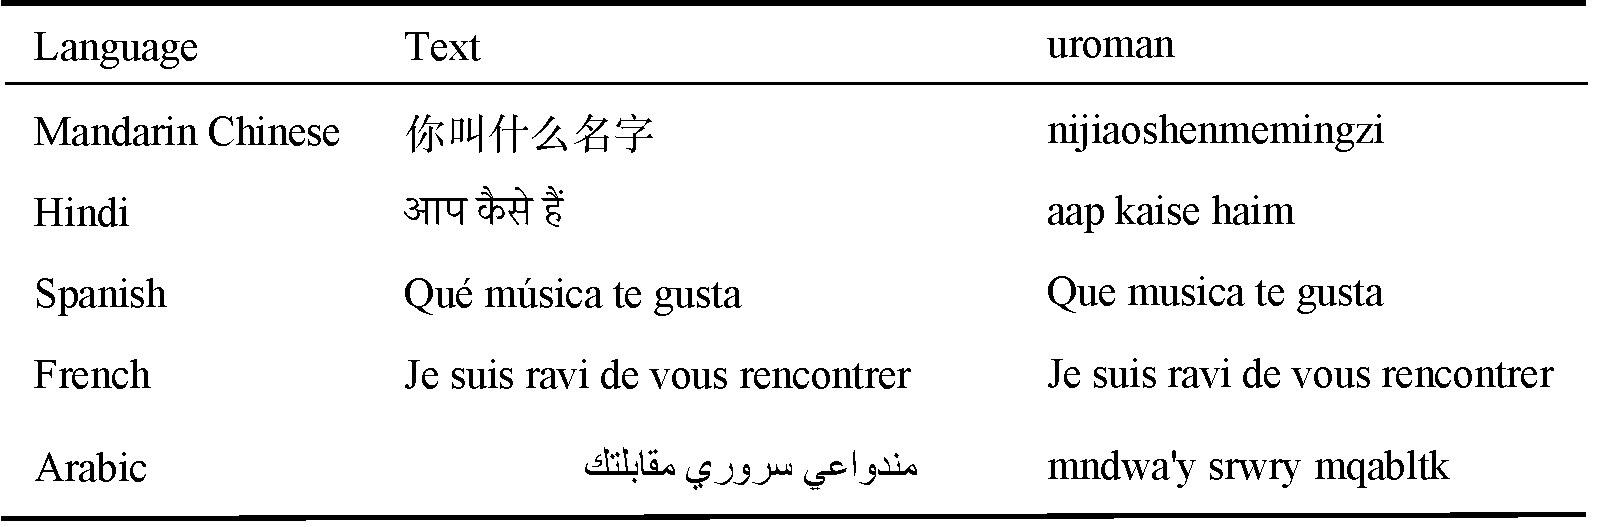
\includegraphics[width=0.75\linewidth]{images/uroman_only2.pdf}
\caption{
\textbf{Illustration of Text Encoding for Forced Alignment.}
Example outputs of uroman~\citep{hermjakob-etal-2018-box}.
} 
\label{tab:data-ex-uroman-xsampa}
\end{table}

}

\newcommand{\insertForceAlignBenchmark}{
\begin{figure}[t]
\centering
\begin{tikzpicture}
\begin{axis}[
width=0.6\textwidth,
height=0.4\textwidth,
% legend style={at={(axis cs:0.5,1200)},anchor=south west},
% , anchor=east,at={(0.93,0.93),draw=none},
% legend cell align={left},
% legend style={},
% legend columns=-1,
% xticklabels from table={\visionEfficiencyTableTrainingTime}{hours},
% xticklabel style={text height=1.5ex},
% xticklabel style={font=\small},
% xtick=data,
% yticklabel style={font=\small},
xtick={0, 100, 500, 1000, 2000},
x tick label style={xshift={(\ticknum==1)*0.7em}},
% xticklabels={$5$,$10$,$15$,$20$,$25$,$30$,$35$,$40$},
% nodes near coords,
% nodes near coords align={vertical},
xmin=0,
ymin=-2,
ymax=100,
% xmin=0,xmax=50,
% bar width=2pt,
ylabel={Wall clock time (sec)},
ylabel near ticks, %ylabel shift={-10pt}
% ylabel style={font=\small},
xlabel={Input audio length (sec)},
xlabel near ticks,
% ymode=log,
% log basis x={2},
% ymode=log,
log ticks with fixed point,
% xlabel style={font=\small},
grid style={dotted,lightgray}
grid=both,
legend style={fill=none, draw=none, at={(0.5,0.91)},anchor=north},
% style=thick,
% xticklabel={$\pgfmathprintnumber{\tick}\%$},
% nodes near coords={\pgfmathprintnumber\pgfplotspointmeta\%}
legend cell align={left},
% legend columns=-1
]

% ctc-segmentation
\addplot[metagray,line width=1,mark=square*,mark options={scale=0.75}, dashed] coordinates {
    % (2, 0.002382)
    % (4, 0.005043)
    % (8, 0.010643)
    % (16, 0.0247)
    % (32, 0.065231)
    % (64, 0.188973)
    % (128, 0.61013)
    % (256, 2.5572)
    % (512, 11.1027)
    % (1024, 47.013395)
    % (2048, 255.2717)
    % (4096, 1429.07014)
    % (8192, 4702.452128)
    (5, 0.060311791)
    % (10, 0.1366108805)
    % (25, 0.450485021)
    % (50, 1.23864168850)
    (100, 3.9413602381)
    % (250, 21.6453406213)
    (500, 94.003602301)
    (1000, 461.9733619)
    (2000, 3080.95882)
    % (3000, 7195.618930)
    % (4000, 10108.36201074)
};
\addplot[metaorange,line width=1.2,mark=triangle*,mark options={scale=1},dashdotted] coordinates {
    % (2, 4.291e-05)
    % (4, 0.00014158)
    % (8, 0.00056212)
    % (16, 0.00239797)
    % (32, 0.0229781)
    % (64, 0.0966518)
    % (128, 0.387659)
    % (256, 1.53957)
    % (512, 6.18548)
    (5, 0.0002211)
    % (10, 0.000898)
    % (25,  0.0117299)
    % (50, 0.0561968)
    (100, 0.228787)
    % (250, 1.41028)
    (500, 5.66702)
    (1000, 22.162)
    (2000, 89.3203)
    % (3000, 195.731)
    % (4000, 371.987)
};


% TorchAudio GPU
\addplot[metablue,line width=1,mark=*,mark options={scale=0.75}] coordinates {
    (5, 0.00272785)
    % (10, 0.0048532535)
    % (25, 0.0120867232279)
    % (50, 0.0299937158776)
    (100, 0.075407437682)
    % (250, 0.328872875091)
    (500, 1.0982227040920)
    (1000, 3.683633243166)
    (2000, 14.5421336991)
    % (3000, 31.36385957344)
    % (4000, 55.42168283648)
    % (5000, 132.800222711)
    % (2, 0.00176)
    % (4, 0.00424)
    % (8, 0.00743)
    % (16, 0.01471)
    % (32, 0.03053)
    % (64, 0.06756)
    % (128, 0.164455)
    % (256, 0.55854)
    % (512, 1.8213)
    % (1024, 6.2817)
    % (2048, 23.904450)
    % (4096, 92.419)
    % (8192, 369.8597)
    
    
};
\legend{ctc-seg (CPU), Flashlight (CPU), MMS (GPU) }
\end{axis}
\end{tikzpicture}
\captionof{figure}{
\textbf{Efficiency of Forced Alignment Implementations.}
The \modelname{} implementation runs on GPU and can process long audio sequences in reasonable time compared to CPU alternatives.
}
\label{fig:results_fa_benchamrk}
% \end{minipage}
\end{figure}

}

\newcommand{\insertStarPlots}{
\begin{figure}
\centering
\begin{subfigure}[l]{.47\textwidth}
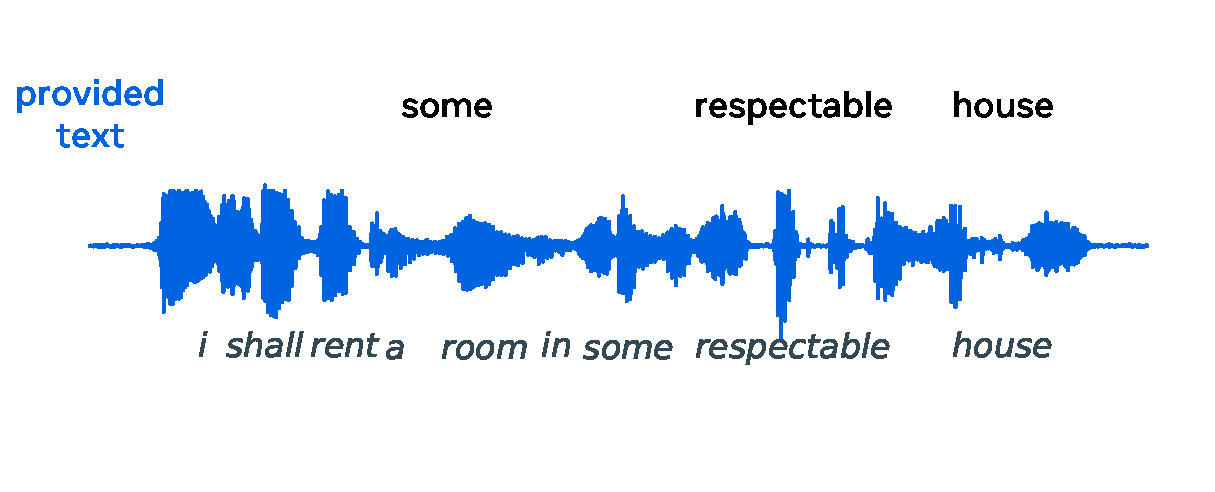
\includegraphics[width=0.99\textwidth,trim={1cm 1cm 1cm 1cm}]{images/star2.pdf}
\end{subfigure}
\begin{subfigure}[l]{.47\textwidth}
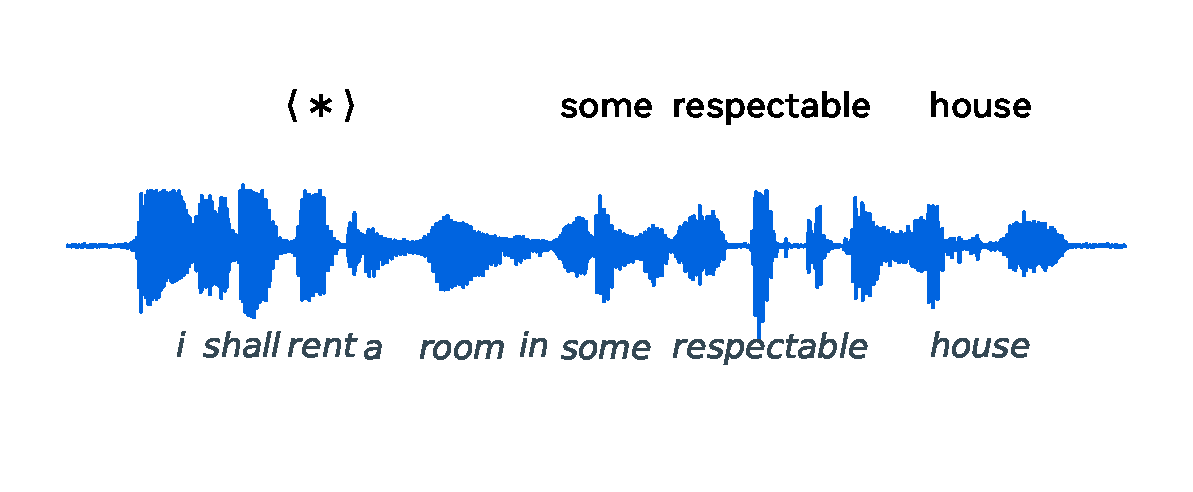
\includegraphics[width=0.99\textwidth,trim={1cm 1cm 1cm 1cm}]{images/star1.pdf} 
\end{subfigure}
\caption{
\textbf{Illustration of the $\Star$ Token in Forced Alignment.}
We show the text to which we would like to align the audio at the top and what is actually spoken at the bottom in italics.
Left: erroneous alignment when the provided text is incomplete. The word \emph{some} is aligned incorrectly.
Right: using $\Star$ token at the beginning enables correct alignment of the provided text.
}
\label{fig:star_token}
\end{figure}
}








\newcommand{\insertTableResultsTTSDesign}{
\begin{table}[t]
\centering
% \resizebox{\linewidth}{!}{
% \begin{small}
\begin{tabular}{lll|rrr|rrr}
\toprule
train & train & text & \multicolumn{3}{c}{ASR (CER)} &  \multicolumn{3}{|c}{MOS} \\
upd & data & repr. & \MMS{} & LJS & FLEURS & \MMS{} & LJS & FLEURS \\
\midrule
\multicolumn{3}{l|}{\emph{Natural speech}} & 4.4 & 4.3 & 9.3 & 3.89	\ci{0.06} & 3.96 \ci{0.06} & 3.37 \ci{0.07} \\
\midrule
800K & LJS & phon. & 5.5 & 4.9 & 5.9 & 3.87 \ci{0.08} & 3.82 \ci{0.06} & 3.73 \ci{0.07} \\
100K & LJS & phon. & 6.3 & 4.9 & 6.3 & 3.64 \ci{0.09} & 3.74 \ci{0.07} & 3.66 \ci{0.07} \\
100K & \MMS{} & phon. & 7.2 & 6.8 & 7.9 & 3.68 \ci{0.07} & 3.51 \ci{0.08} & 3.54 \ci{0.07} \\
100K & \MMS{} & chars & 7.2	& 9.2 & 10.0 & 3.58 \ci{0.08} & 3.45 \ci{0.08} & 3.34 \ci{0.09} \\
\bottomrule
\end{tabular}
% \end{small}
% }
\vspace{1mm}
\caption{
\textbf{Ablation of Training Setup.} 
Our design choices (last row) lead to a moderate quality reduction compared to the standard VITS setup (second row) but enable scaling TTS to \nummmslang{} languages.
The standard VITS setting performs 800K training updates on clean LJSpeech data using a high quality phonemizer while as \modelname{} is trained on \MMS{} data for fewer updates and with characters.
Natural speech results are based on the human utterances of each dataset.
We report ASR CER and MOS scores from a human study with confidence interval 95\% on the English development sets of \MMS{}, LJSpeech and FLEURS.
} 
\label{tab:tts-design}
\end{table}
}


\newcommand{\insertTableResultsTTSDrama}{
\begin{table}[t]
\centering
% \resizebox{\linewidth}{!}{
\begin{tabular}{l|rrr|rrr}
\toprule
& \multicolumn{3}{c|}{ASR (CER)} & \multicolumn{3}{c}{MOS} \\
& \MMS{} & LJS & FLEURS & \MMS{} & LJS & FLEURS \\
\midrule
\emph{Natural speech} & 4.4 & 4.3 & 9.3 & 3.89 \ci{0.06} & 3.96 \ci{0.06} & 3.37 \ci{0.07} \\
no background music & 7.2 & 9.2 & 10.0 & 3.51 \ci{0.07} & 3.52 \ci{0.08} & 3.41 \ci{0.09} \\
\midrule
background music & 11.8 & 15.6 & 16.1 & 3.24 \ci{0.08} & 2.98 \ci{0.08} & 3.01 \ci{0.08} \\
\hspace{2mm}+ denoise & 10.8 & 13.2 & 14.4 & 3.32 \ci{0.08} & 3.18 \ci{0.07} & 3.16 \ci{0.08} \\
\hspace{2mm}+ denoise + filter & 7.8 & 10.8 & 11.9 & 3.47 \ci{0.07} & 3.32 \ci{0.08} & 3.12 \ci{0.07} \\
\bottomrule
\end{tabular}
% }
\vspace{1mm}
\caption{
\textbf{Ablation of Building TTS Models using Data with Background Music.}
Curating the training data containing background music results in TTS systems which approach the performance of models trained on recordings without background music. 
We show MOS ratings as well as ASR CER on three different benchmarks for English data for the development sets of \MMS{}, LJSpeech and FLEURS.
The TTS model labeled "no background music" is identical to the last row in~\autoref{tab:tts-design} and we use the \MMS{} development set of the non-drama recording.
} 
\label{tab:tts-drama}
\end{table}
}



\newcommand{\insertTableResultsTTSFLEURS}{
\begin{table}
\centering
% \resizebox{\linewidth}{!}{
\begin{tabular}{lrrrr}
\toprule
& \multicolumn{2}{c}{ASR (CER)} & \multicolumn{2}{c}{MOS} \\
& TTS & ref & TTS & ref \\
\midrule
In-domain     & 11.1 & 9.2 & 3.51 {\tiny $\pm$ 0.11} & 3.61 {\tiny $\pm$ 0.11} \\
Out-of-domain & 11.3 & 8.8 & 3.52 {\tiny $\pm$ 0.11} & 3.33	{\tiny $\pm$ 0.12}$^*$ \\
\bottomrule
\end{tabular}
% }
\vspace{1mm}
\caption{
\textbf{TTS in-domain and Out-of-domain Evaluation on 61 Languages.}
We synthesize the test sets of \MMS{} (in-domain) and FLEURS (out-of-domain) to measure character error rate (CER) and collect human judgements (MOS) for both the model outputs (TTS) and human utterances (ref). 
The \modelname{} models are robust with little performance degradation when applied to general domain data (out-of-domain):
they retain much of the original content (low difference between CER of TTS and ref) and the systems produce outputs with good prosody and sound quality (low difference between MOS scores between TTS and ref).
We show MOS scores with confidence interval 95\%.
($^*$) human judges assigned low ratings since the human reference audio in FLEURS contains a lot of variability compared to synthesized speech or the \MMS{} reference speech (in-domain ref).
} 
\label{tab:tts-fleurs}
\end{table}
}

\newcommand{\insertTableResultsTTSFull}{
\begin{table}
\centering
% \resizebox{\linewidth}{!}{
\begin{tabular}{lrrrrrr}
\toprule
& \#lang & MCD & \multicolumn{2}{c}{ASR (CER)} & TTS CER & \% \\
& & & TTS & ref & $\leq$ 5 & \\
\midrule
Asia & 335 & 4.30 \ci{0.1} & 3.1 \ci{0.2} & 1.9 \ci{0.1} & 296 & 88\% \\
South America & 136 & 4.10 \ci{0.1} & 2.6 \ci{0.2} & 1.8 \ci{0.1} & 129 & 95\% \\
North America & 144 & 4.12 \ci{0.1} & 3.8 \ci{0.8} & 2.4 \ci{0.2} & 125 & 87\% \\
Europe & 41 & 4.33 \ci{0.2} & 3.0 \ci{0.3} & 1.9 \ci{0.2} & 39 & 95\% \\
Africa & 363 & 4.34 \ci{0.1} & 4.1 \ci{0.2} & 2.6 \ci{0.1} & 277 & 76\% \\
Pacific & 88 & 4.72 \ci{0.2} & 3.4 \ci{1.3} & 1.8 \ci{0.2} & 79 & 90\% \\
\midrule
& 1,107 & 4.30 \ci{0.0} & 3.5 \ci{0.2} & 2.2 \ci{0.1} & 945 & 85\% \\
\bottomrule
\end{tabular}
% }
\vspace{1mm}
\caption{
\textbf{TTS Evaluation on \nummmslang{} Languages.}
The majority of \modelname{} TTS models can synthesize speech which preserves most of the content as per the ASR character error rates (TTS CER $\leq$ 5).
We report MCD and character error rate for the synthesized outputs (TTS) of the \MMS{} test sets as well as the human references (ref).
We also show the number of systems which achieve CER less than five, indicating systems which on average produce no more than one incorrect character every twenty characters.
Results are shown with confidence interval 95\%.
} 
\label{tab:tts-full}
\end{table}
}



\newcommand{\insertResultsASRWisper}{
\begin{table}[]
\centering
\begin{tabular}{lrrrr}
\toprule
& \#lang & labeled train & \multicolumn{2}{c}{FLEURS-54} \\
& & data (h) & dev & test \\
\midrule
\textit{Prior Work} \\
Whisper medium & 99 & 680K & - & 50.1 \\
Whisper large-v2 & 99 & 680K & - & 44.3 \\
\midrule
\textit{This Work} \\
\modelname{} & 61 & 3K & 20.9 & 20.7 \\
\modelname{} (LSAH) & 61 & 3K & 19.0 & 19.1 \\
\modelname{} & \nummmslang{} & \nummmshrsrd{} & 24.8 & 24.8 \\
\modelname{} (LSAH) & 1,107 & \nummmshrsrd{} & 18.7 & 18.7 \\
\bottomrule
\end{tabular}
\vspace{1mm}
\caption{
\textbf{Comparison to Whisper.} 
We report average WER on the 54 languages of the FLEURS benchmark supported by both Whisper and \modelname{} (FLEURS-54).
\modelname{} is a CTC-based model and to enable a fairer comparison we use n-gram models trained on web data when comparing to Whisper whose decoder is a neural sequence-model that serves as a language model and was trained on billions of web tokens. 
% Appendix~\ref{app:asr-whisper} provides a per language breakdown and additional results.
} 
\label{tab:asr-whisper} 
\end{table}
}



\newcommand{\insertResultsASRWisperFull}{
\begin{table}[t]
\centering
\begin{tabular}{lrrrrr}
\toprule
& \#lang & lbld train & \multicolumn{2}{c}{FLEURS-54} \\
& & data (h) & (M) & dev & test \\
\midrule
\textit{Prior Work} \\
Whisper medium & 99 & \multirow{2}{*}{680K} & 769M & - & 50.1 \\
Whisper large-v2 & 99 & & 1,550M & - & 44.3 \\
\midrule
\textit{This Work} \\
\modelname{} & 61 & 3K & 965M & 33.6 & 33.3 \\
\hspace{2mm} + CC LM & 61 & 3K & 965M & 20.9	& 20.7\\ 
\modelname{} (LSAH) & 61 & 3K & 1,096M & 31.4	& 31.0 \\
\hspace{2mm} + CC LM & 61 & 3K &  1,096M & 19.1 & 19.0\\
\midrule
\modelname{} & \nummmslang{} & \nummmshrsrd{} & 965M & 44.7 &	44.2 \\
\hspace{2mm} + CC LM  & \nummmslang{} & \nummmshrsrd{} & 965M & 24.8 &	24.8 \\
\modelname{} (LSAH) & 1,107 & \nummmshrsrd{} & 3,346M & 32.8  &	32.5 \\
\hspace{2mm} + CC LM  & 1,107 & \nummmshrsrd{} & 3,346M & 18.7 & 18.7 \\
\bottomrule
\end{tabular}
\vspace{1mm}
\caption{
\textbf{Comparison to Whisper.} 
We report average WER on the 54 languages of the FLEURS benchmark supported by both Whisper and \modelname{} (FLEURS-54).
\modelname{} is a CTC-based model and to enable a fairer comparison we use n-gram models trained on web data when comparing to Whisper whose decoder is a neural sequence-model and serves as a language model that was trained on billions of web tokens. 
} 
\label{tab:asr-whisper-full} 
\end{table}
}


\newcommand{\insertResultsASRWisperPerLang}{
\begin{table}[h!]
\centering
\begin{scriptsize}
\begin{tabular}{lrrrrrrrrrrrr}
\toprule
& Whisper & Whisper & \modelname{} & \modelname{} & \modelname{} & \modelname{} & \modelname{} & \modelname{} & \modelname{} & \modelname{} \\
& medium & large-v2 & L-61 & L-61 & L-61 & L-61 & L-1107 & L-1107 & L-1107 & L-1107 \\
&  &  & noLM & CC LM & noLM & CC LM & noLM & CC LM & noLM & CC LM \\
&  &  &  &  & LSAH & LSAH &  &  & LSAH & LSAH \\
\midrule
Amharic & 229.3 & 140.3 & 48.7 & 30.7 & 52.4 & 32.5 & 52.9 & 30.1 & 53.3 & 31.1\\
Arabic & 20.4 & 16.0 & 34.9 & 19.6 & 35.8 & 19.9 & 44.0 & 23.4 & 41.3 & 21.0\\
Assamese & 102.3 & 106.2 & 29.5 & 18.8 & 28.4 & 18.6 & 37.6 & 21.2 & 30.5 & 19.2\\
Azerbaijani & 33.1 & 23.4 & 40.7 & 21.3 & 38.3 & 19.8 & 45.0 & 21.2 & 40.1 & 19.1\\
Bengali & 100.6 & 104.1 & 19.7 & 11.6 & 20.0 & 12.1 & 25.0 & 12.5 & 23.5 & 12.1\\
Bulgarian & 21.4 & 14.6 & 23.4 & 13.1 & 23.9 & 13.3 & 27.9 & 12.9 & 25.5 & 13.5\\
Burmese & 123.0 & 115.7 & 22.2 & 14.2 & 22.3 & 14.5 & 29.2 & 20.2 & 24.5 & 16.0\\
Catalan & 9.6 & 7.3 & 18.1 & 11.0 & 18.1 & 11.0 & 25.9 & 11.5 & 20.1 & 10.8\\
Dutch & 9.9 & 6.7 & 26.9 & 13.7 & 26.4 & 14.3 & 38.1 & 14.9 & 27.6 & 14.5\\
English & 4.4 & 4.2 & 23.8 & 10.7 & 24.8 & 11.8 & 38.8 & 12.2 & 27.8 & 12.3\\
Filipino & 19.1 & 13.8 & 19.3 & 11.9 & 19.4 & 12.2 & 26.2 & 13.5 & 20.2 & 12.4\\
Finnish & 13.9 & 9.7 & 26.4 & 22.5 & 26.9 & 23.1 & 32.3 & 22.2 & 28.8 & 23.1\\
French & 8.7 & 8.3 & 24.3 & 13.7 & 24.5 & 14.1 & 35.8 & 15.4 & 29.3 & 15.0\\
German & 6.5 & 4.5 & 22.5 & 13.2 & 22.3 & 13.7 & 38.4 & 13.1 & 22.5 & 13.3\\
Greek & 19.0 & 12.5 & 40.8 & 14.0 & 40.5 & 13.6 & 57.5 & 13.0 & 40.1 & 13.6\\
Gujarati & 104.8 & 102.7 & 23.0 & 13.0 & 22.7 & 12.8 & 73.9 & 56.4 & 24.0 & 12.8\\
Hausa & 106.6 & 88.9 & 35.9 & 26.7 & 36.3 & 27.3 & 40.4 & 26.7 & 38.3 & 26.4\\
Hebrew & 33.1 & 27.1 & 68.5 & 44.8 & 66.6 & 41.5 & 78.7 & 50.9 & 67.1 & 40.0\\
Hindi & 26.8 & 21.5 & 65.0 & 44.4 & 28.8 & 16.0 & 70.7 & 45.7 & 21.2 & 10.6\\
Hungarian & 24.3 & 17.0 & 31.2 & 18.1 & 30.7 & 18.4 & 40.3 & 18.3 & 30.7 & 18.0\\
Icelandic & 49.9 & 38.2 & 42.9 & 18.3 & 42.3 & 19.9 & 53.6 & 20.5 & 45.3 & 18.6\\
Indonesian & 10.2 & 7.1 & 25.5 & 11.7 & 23.8 & 12.1 & 31.9 & 11.6 & 23.4 & 11.8\\
Javanese & 67.9 & 68.5 & 32.8 & 19.6 & 32.8 & 20.0 & 58.8 & 27.2 & 34.2 & 19.5\\
Kannada & 77.7 & 37.0 & 18.8 & 14.4 & 15.8 & 12.9 & 41.3 & 25.2 & 17.7 & 13.3\\
Kazakh & 48.8 & 37.7 & 30.2 & 17.4 & 30.2 & 17.7 & 63.8 & 19.5 & 31.6 & 17.4\\
Khmer & 103.8 & 128.9 & 26.0 & 19.9 & 25.7 & 19.8 & 70.7 & 52.4 & 26.7 & 19.7\\
Korean & 16.4 & 14.3 & 58.7 & 37.5 & 59.9 & 37.3 & 82.1 & 58.2 & 68.3 & 40.1\\
Lao & 101.4 & 101.5 & 48.9 & 45.4 & 24.2 & 22.8 & 62.1 & 56.6 & 22.6 & 16.9\\
Latvian & 32.0 & 23.1 & 20.8 & 12.0 & 20.9 & 12.1 & 24.5 & 11.9 & 21.8 & 12.1\\
Malay & 12.2 & 8.7 & 25.3 & 12.3 & 25.9 & 13.2 & 32.4 & 12.1 & 26.1 & 12.5\\
Malayalam & 101.1 & 100.7 & 23.7 & 19.1 & 19.5 & 16.6 & 39.1 & 25.6 & 20.4 & 15.3\\
Marathi & 63.2 & 38.3 & 32.5 & 19.0 & 19.2 & 13.5 & 28.0 & 14.9 & 20.9 & 13.4\\
Mongolian & 103.7 & 110.5 & 55.7 & 29.3 & 54.9 & 32.9 & 67.7 & 28.7 & 55.3 & 32.3\\
Persian & 41.0 & 32.9 & 39.7 & 22.9 & 39.9 & 22.5 & 44.4 & 21.3 & 42.9 & 22.0\\
Polish & 8.0 & 5.4 & 21.5 & 11.4 & 20.8 & 11.6 & 33.0 & 11.0 & 25.1 & 11.3\\
Portuguese & 5.0 & 4.3 & 16.1 & 10.8 & 16.3 & 10.8 & 19.3 & 10.2 & 17.7 & 10.5\\
Punjabi & 102.0 & 102.4 & 41.4 & 29.9 & 30.4 & 20.7 & 99.0 & 91.0 & 31.0 & 19.8\\
Romanian & 20.0 & 14.4 & 27.9 & 18.8 & 28.4 & 19.1 & 31.3 & 17.8 & 27.4 & 18.3\\
Russian & 7.2 & 5.6 & 30.3 & 14.6 & 30.4 & 14.3 & 38.8 & 14.7 & 35.0 & 15.0\\
Shona & 143.9 & 121.0 & 38.1 & 30.4 & 37.7 & 30.1 & 43.0 & 29.9 & 37.8 & 29.6\\
Somali & 104.0 & 102.9 & 51.8 & 42.8 & 52.5 & 43.0 & 54.5 & 42.9 & 53.8 & 42.8\\
Spanish & 3.6 & 3.0 & 12.2 & 7.8 & 12.4 & 8.2 & 14.0 & 7.8 & 14.0 & 8.7\\
Swahili & 52.8 & 39.3 & 22.9 & 16.0 & 23.3 & 15.6 & 29.6 & 16.8 & 23.7 & 16.0\\
Swedish & 11.2 & 8.5 & 29.9 & 17.4 & 30.5 & 17.5 & 38.2 & 17.2 & 33.5 & 17.4\\
Tajik & 74.0 & 85.8 & 59.8 & 46.6 & 33.9 & 19.2 & 59.0 & 39.5 & 25.7 & 15.7\\
Tamil & 23.1 & 17.5 & 24.2 & 18.3 & 21.9 & 16.3 & 25.3 & 17.3 & 23.9 & 16.3\\
Telugu & 82.8 & 99.0 & 19.4 & 13.7 & 19.6 & 13.7 & 24.5 & 15.8 & 22.1 & 13.6\\
Thai & 15.4 & 11.5 & 18.2 & 13.6 & 18.1 & 13.6 & 27.6 & 18.8 & 20.7 & 14.3\\
Turkish & 10.4 & 8.4 & 28.6 & 17.3 & 28.7 & 17.5 & 31.2 & 16.1 & 30.9 & 16.9\\
Ukrainian & 11.6 & 8.6 & 31.1 & 13.6 & 31.7 & 13.5 & 39.2 & 13.3 & 33.3 & 13.6\\
Urdu & 28.2 & 22.6 & 42.3 & 22.7 & 33.1 & 20.1 & 46.4 & 25.1 & 36.9 & 20.5\\
Vietnamese & 12.7 & 10.3 & 44.5 & 18.6 & 47.5 & 20.7 & 56.6 & 21.0 & 52.9 & 19.8\\
Welsh & 40.8 & 33.0 & 48.9 & 20.8 & 49.0 & 20.8 & 54.9 & 21.4 & 51.4 & 20.9\\
Yoruba & 105.1 & 94.8 & 61.2 & 49.7 & 61.9 & 49.4 & 62.7 & 50.2 & 64.2 & 49.4\\
\midrule 
& 50.1 & 44.3 & 33.3 & 20.7 & 31.0 & 19.1 & 44.2 & 24.8 & 32.5 & 18.7\\
\bottomrule
\end{tabular}
\end{scriptsize}
\vspace{1mm}
\caption{
\textbf{Comparison to Whisper on the FLEURS test set.}
We report WER for each of the 54 languages supported by both \modelname{} and Whisper, except for Thai (tha), Lao (lao), Burmese (mya) and Khmer (khm) where we report CER. 
We apply Whisper normalization for both reference and hypothesis for measuring CER/WER.
} 
\label{tab:asr-whisper-perlang-test} 
\end{table}
}


\newcommand{\insertResultsASRUSM}{
\begin{table}[t]
\centering
\begin{tabular}{lrr}
\toprule
& \multicolumn{2}{c}{FLEURS-102} \\
& dev & test \\
\midrule
\textit{Prior Work} \\
w2v-BERT~\citep{chen2022maestro} & - & 12.3 \\
Maestro-U~\citep{chen2022maestro} & - & 8.7 \\
USM~\citep{zhang2023usm} & - & 6.9 \\
USM-M~\citep{zhang2023usm} & - & 6.5 \\
USM-M-adapter~\citep{zhang2023usm} & - & 6.7 \\
\midrule
\textit{This Work} \\
% \modelname{} FL-102 & 7.7 & 7.6 \\
\modelname{} FL-102 (LSFT) + LM & 6.3 & 6.3 \\
% ASR-all & 127 & & \\
% ASR-all & \nummmslang{} & & \\
\bottomrule
\end{tabular}
\vspace{1mm}
\caption{
\textbf{Comparison to Google USM.} 
We report average CER on the 102 languages of FLEURS and use n-gram models together with our CTC acoustic models.
USM-M is an RNN-T model which uses both unlabeled text as well as labeled speech data during pre-training and for \modelname{} we use unlabeled text to train language models for inference.
}
\label{tab:asr-usm}
\end{table}
}



\newcommand{\insertPretainXLSRvsMMS}{

\pgfplotstableread[row sep=\\,col sep=&]{
lang & delta \\
amh & 7.94 \\
lao & 6.57 \\
mal & 5.63 \\
nya & 4.95 \\
swh & 2.62 \\
ful & 2.12 \\
kor & 2.11 \\
pan & 2 \\
lug & 1.97 \\
urd & 1.42 \\
khm & 1.41 \\
mar & 1.4 \\
hin & 1.38 \\
orm & 1.34 \\
tel & 1.27 \\
hau & 1.23 \\
tam & 1.23 \\
guj & 1.04 \\
vie & 0.87 \\
mya & 0.82 \\
jav & 0.76 \\
asm & 0.72 \\
azj & 0.69 \\
tha & 0.57 \\
som & 0.5 \\
ben & 0.43 \\
kaz & 0.39 \\
tgl & 0.28 \\
yor & 0.28 \\
heb & 0.22 \\
zlm & 0.21 \\
ceb & 0.2 \\
ind & 0.2 \\
tur & 0.17 \\
mon & 0.11 \\
ory & 0.11 \\
kan & 0.06 \\
fin & 0.02 \\
nld & -0.01 \\
sna & -0.03 \\
bul & -0.06 \\
ron & -0.14 \\
ara & -0.22 \\
ukr & -0.24 \\
pol & -0.24 \\
lav & -0.25 \\
kir & -0.26 \\
deu & -0.26 \\
cat & -0.28 \\
hun & -0.29 \\
swe & -0.36 \\
por & -0.39 \\
fas & -0.48 \\
fra & -0.51 \\
rus & -0.54 \\
eng & -0.64 \\
ell & -0.66 \\
spa & -0.7 \\
isl & -1.14 \\
tgk & -1.72 \\
cym & -1.87 \\
}\dataDelta 
\begin{figure}
\centering
  % \resizebox{.95\linewidth}{!}{%
\begin{tikzpicture}
\begin{axis}[
width=1*\textwidth,
height=.4\textwidth,
ylabel={CER \modelname{}} - XLS-R,
ylabel style={align=center,text width=5cm},
legend style={%font=\small,
at={(0.88,0.87)},
minor tick num=1,
% grid=both,
% grid style={line width=.5pt, draw=gray!10},
% major grid style={line width=.2pt,draw=gray!50},
anchor=east,legend columns=4,draw=none},
ymin=-5,
ymax=10,
xticklabels from table={\dataDelta}{lang},
x tick label style={rotate=45,font=\tiny},
enlarge x limits=0,
xtick=data]
\addplot[solid,metablue,line width=0.6,mark=*,mark options={solid, scale=0.4}] table[xticklabels from table={\dataDelta}{lang},x expr=\coordindex,x=lang,y=delta]{\dataDelta};
\addplot[color=gray,dashed] coordinates {(0,0) (61,0)};
\end{axis}
\end{tikzpicture}
% }
\caption{
\textbf{\modelname{} vs. XLS-R Breakdown.}
We show the absolute character error rate difference between multilingual ASR models based on XLS-R and \modelname{} models with 1B parameters.
Positive values indicate better performance of \modelname{} and negative values better performance of XLS-R.
Models are fine-tuned on \MMS{} data and evaluated on the development sets of 61 FLEURS languages.
}
\label{fig:pretrain-xlsr-mms-perlang}
\end{figure}
}


\newcommand{\insertResultsGenderBiasFull}{
\begin{table}[h!]
\centering
% \begin{scriptsize}
\begin{tabular}{l|rr|rrr|rrr}
\toprule
& \multicolumn{2}{c}{Num Samples} & \multicolumn{3}{c}{\modelname{} ASR CER $\downarrow$} & \multicolumn{3}{c}{FLEURS ASR CER $\downarrow$}  \\
& Female & Male & Female & Male & Overall & Female & Male & Overall \\
\midrule
Assamese & 139 & 279 & 15.3 & 15.1 & 15.4 & 8.6 & 8.0 & 8.9 \\
Bulgarian & 189 & 206 & 9.0 & 10.2 & 7.9 & 3.6 & 3.5 & 3.6 \\
Welsh & 150 & 296 & 15.8 & 19.4 & 14.1 & 8.4 & 11.5 & 6.9 \\
Greek & 125 & 146 & 11.4 & 9.3 & 13.1 & 5.4 & 4.0 & 6.6 \\
English & 245 & 149 & 10.8 & 10.7 & 10.9 & 6.0 & 5.5 & 6.8 \\
Spanish & 130 & 278 & 5.2 & 5.8 & 5.0 & 2.3 & 2.9 & 2.0 \\
Fula & 107 & 166 & 27.2 & 29.0 & 26.2 & 14.8 & 21.4 & 11.0 \\
Finnish & 352 & 63 & 7.6 & 7.1 & 10.2 & 2.7 & 2.6 & 3.8 \\
French & 62 & 227 & 9.1 & 10.0 & 8.8 & 5.4 & 6.4 & 5.2 \\
Gujarati & 149 & 283 & 13.3 & 12.7 & 13.7 & 6.2 & 6.2 & 6.2 \\
Hindi & 120 & 119 & 15.1 & 15.5 & 14.7 & 6.6 & 8.3 & 5.1 \\
Kazakh & 136 & 232 & 7.8 & 7.4 & 8.0 & 3.1 & 2.4 & 3.6 \\
Khmer & 98 & 228 & 26.1 & 22.8 & 27.6 & 14.1 & 11.2 & 15.4 \\
Kannada & 245 & 123 & 10.0 & 10.4 & 9.3 & 5.2 & 5.2 & 5.1 \\
Korean & 93 & 133 & 24.3 & 26.0 & 22.9 & 13.5 & 14.0 & 13.1 \\
Kyrgyz & 273 & 149 & 10.6 & 12.1 & 7.9 & 4.5 & 5.7 & 2.1 \\
Ganda & 228 & 78 & 13.4 & 13.3 & 13.6 & 8.2 & 7.9 & 9.0 \\
Latvian & 177 & 179 & 7.0 & 6.6 & 7.3 & 3.0 & 2.7 & 3.3 \\
Marathi & 148 & 295 & 13.2 & 9.3 & 15.0 & 8.2 & 4.8 & 9.9 \\
Polish & 95 & 243 & 6.6 & 7.2 & 6.3 & 3.3 & 3.8 & 3.1 \\
Russian & 203 & 153 & 8.0 & 7.4 & 8.9 & 4.0 & 3.7 & 4.6 \\
Shona & 118 & 275 & 10.5 & 8.6 & 11.4 & 4.1 & 2.2 & 5.1 \\
Swedish & 64 & 266 & 10.1 & 8.5 & 10.5 & 5.6 & 4.6 & 5.9 \\
Swahili & 59 & 152 & 7.7 & 11.1 & 6.5 & 3.7 & 3.9 & 3.6 \\
Tamil & 214 & 163 & 15.3 & 17.0 & 13.2 & 8.9 & 10.1 & 7.4 \\
Telugu & 76 & 235 & 12.7 & 11.3 & 13.1 & 7.9 & 8.2 & 7.8 \\
Tajik & 116 & 123 & 11.1 & 12.5 & 9.9 & 4.3 & 4.9 & 3.7 \\
\midrule
Average & - & - & 12.4 & 12.3 & 12.4 & 6.5 & 6.2 & 6.4 \\
\bottomrule
\end{tabular}
% \end{scriptsize}
\vspace{1mm}
\caption{
\textbf{Analysis of Gender Bias.}
We compare ASR models trained on \MMS{} data and FLEURS data.
We report dev CER per gender of the speakers for 27 languages of FLEURS for which \MMS{} provides data and for which there are at least 50 samples for each gender. 
}
\label{tab:rai-gender-full-results} 
\end{table}
}

\newcommand{\insertTableASREverything}{
\begin{table}[t]
\centering
\begin{tabular}{lrrrrr}
\toprule
& \#lang & FLEURS & CV & VP & MLS \\
\midrule
\textit{Prior Work} \\
VoxPopuli~\citep{wang2021voxpopuli} & 1 & & & 15.3 \\
Maestro~\citep{chen2022maestro}  & 14 & & & 8.1 \\
RNN-T 1B~\citep{boli2021scaling} & 15 & & & & 7.9 \\
Whisper~\citep{radford2022whisper} & 99 & & & 13.6$^*$ & 7.3* \\
ML-IO~\citep{tjandra2022massively} & 70 & & & & 7.5 \\
USM-M~\citep{zhang2023usm} & 102 & 6.5 \\
\midrule
\textit{This Work - Single-Domain training} \\
FL & 102 & 6.4 & & & \\
CV & 76 & & 19.7 & & \\
VP & 14 & & & 10.3 & \\
MLS & 8 & & & & 8.7 \\
\midrule
\textit{This Work - Multi-Domain training} \\
\MMS{}+FL+CV+VP+MLS & 1,162 & 6.2 & 19.6 & 10.6 & 9.0 \\
\bottomrule
\end{tabular}
\vspace{1mm}
\caption{
\textbf{Evaluation of \modelname{} on Multilingual Benchmarks.} 
\modelname{} is fine-tuned on \MMS{}, FLEURS, CommonVoice, Voxpopuli and MLS. 
We report CER on FLEURS and WER on the other benchmarks.
Results are averaged over all languages of a benchmark and $^{(*)}$ indicates results with a different data normalization which does not enable a strict comparison to other results~\citep{radford2022whisper}.
Our models use n-gram language models trained on Common Crawl during inference.
For each approach, we show the number of languages an individual models supports and some prior results are based on multiple models, e.g., \citet{wang2021voxpopuli}.
} 
\label{tab:asr-everything}
\end{table}
}

\newcommand{\insertResultsASRUSMFull}{
\begin{table}[h!]
\centering
\begin{small}
\begin{minipage}[t]{0.49\textwidth}
\begin{tabular}{lrrrr}
\toprule
& Dev  &  Test   & LM    \\
& CER  &  CER   &     \\
\midrule
Afrikaans & 6.3 & 6.3 & CC LM \\
Amharic & 6.8 & 7.0 & CC LM \\
Arabic & 4.3 & 4.9 & CC LM \\
Assamese & 7.3 & 7.7 & CC LM \\
Asturian & 5.2 & 5.1 & CC LM \\
Azerbaijani & 4.2 & 3.9 & CC LM \\
Belarusian & 3.8 & 3.8 & CC LM \\
Bengali & 5.1 & 5.3 & CC LM \\
Bosnian & 3.8 & 3.4 & FL LM \\
Bulgarian & 3.0 & 3.2 & CC LM \\
Catalan & 2.8 & 2.9 & CC LM \\
Cebuano & 3.6 & 4.4 & CC LM \\
Czech & 3.3 & 3.0 & CC LM \\
Sorani & 6.5 & 7.4 & FL LM \\
Mandarin & 14.8 & 14.9 & CC LM \\
Welsh & 5.7 & 5.9 & CC LM \\
Danish & 5.5 & 5.7 & CC LM \\
German & 3.0 & 2.7 & CC LM \\
Greek & 4.0 & 3.7 & CC LM \\
English & 4.6 & 4.3 & CC LM \\
Estonian & 2.9 & 2.7 & FL LM \\
Persian & 4.0 & 4.1 & FL LM \\
Finnish & 2.6 & 2.4 & FL LM \\
French & 4.1 & 4.1 & CC LM \\
Fula & 13.9 & 13.8 & FL LM \\
Irish & 19.3 & 19.5 & CC LM \\
Galician & 2.8 & 2.7 & CC LM \\
Gujarati & 5.2 & 5.1 & CC LM \\
Hausa & 5.5 & 5.9 & CC LM \\
Hebrew & 15.5 & 12.9 & CC LM \\
Hindi & 5.4 & 4.7 & CC LM \\
Croatian & 3.5 & 3.2 & CC LM \\
Hungarian & 4.1 & 4.2 & CC LM \\
Armenian & 3.2 & 3.2 & FL LM \\
Igbo & 10.7 & 11.1 & FL LM \\
Indonesian & 2.3 & 2.1 & CC LM \\
Icelandic & 5.2 & 4.1 & CC LM \\
Italian & 1.5 & 1.4 & CC LM \\
Javanese & 4.3 & 3.8 & CC LM \\
Japanese & 14.5 & 14.6 & CC LM \\
Kamba & 12.5 & 11.3 & FL LM \\
Kannada & 4.6 & 4.4 & FL LM \\
Georgian & 3.4 & 3.6 & CC LM \\
Kazakh & 2.9 & 3.1 & CC LM \\
Kabuverdianu & 4.3 & 4.3 & FL LM \\
Khmer & 9.9 & 10.3 & CC LM \\
Kyrgyz & 4.1 & 3.6 & FL LM \\
Korean & 11.4 & 11.8 & CC LM \\
Lao & 26.5 & 24.1 & CC LM \\
Latvian & 2.8 & 2.2 & CC LM \\
Lingala & 4.0 & 4.3 & FL LM \\
Lithuanian & 4.3 & 3.7 & CC LM \\
% \vdots & \vdots & \vdots & \vdots \\ 
\bottomrule
\end{tabular}
\end{minipage} \hfill
\begin{minipage}[t]{0.49\textwidth}
\begin{tabular}{lrrrr}
\toprule
& Dev  &  Test   & LM    \\
& CER  &  CER   &     \\
\midrule
% \vdots & \vdots & \vdots & \vdots \\ 
Luxembourgish & 8.0 & 7.5 & CC LM \\
Ganda & 8.0 & 8.4 & FL LM \\
Luo & 4.9 & 5.0 & FL LM \\
Malayalam & 4.4 & 4.2 & FL LM \\
Marathi & 7.2 & 6.6 & CC LM \\
Macedonian & 2.0 & 1.9 & CC LM \\
Maltese & 3.7 & 3.7 & CC LM \\
Mongolian & 5.6 & 5.9 & CC LM \\
Maori & 5.9 & 6.9 & CC LM \\
Burmese & 8.9 & 9.2 & CC LM \\
Dutch & 3.7 & 3.1 & CC LM \\
Norwegian & 3.7 & 4.1 & CC LM \\
Nepali & 8.3 & 7.7 & CC LM \\
Northern & 6.8 & 6.1 & FL LM \\
Nyanja & 6.3 & 6.7 & CC LM \\
Occitan & 7.8 & 8.2 & CC LM \\
Oromo & 15.7 & 16.2 & CC LM \\
Oriya & 6.3 & 7.1 & CC LM \\
Punjabi & 7.4 & 7.0 & CC LM \\
Polish & 2.6 & 2.7 & CC LM \\
Portuguese & 2.8 & 2.8 & CC LM \\
Pashto & 13.1 & 14.1 & CC LM \\
Romanian & 3.7 & 3.1 & CC LM \\
Russian & 3.1 & 3.0 & CC LM \\
Slovak & 2.7 & 2.5 & CC LM \\
Slovenian & 4.0 & 3.7 & CC LM \\
Shona & 3.8 & 4.1 & FL LM \\
Sindhi & 7.2 & 7.2 & FL LM \\
Somali & 12.8 & 13.0 & CC LM \\
Spanish & 1.8 & 2.1 & CC LM \\
Serbian & 10.3 & 12.7 & FL LM \\
Swedish & 4.7 & 4.6 & CC LM \\
Swahili & 3.3 & 3.4 & CC LM \\
Tamil & 8.2 & 9.0 & FL LM \\
Telugu & 6.6 & 6.9 & CC LM \\
Tajik & 4.0 & 4.5 & CC LM \\
Filipino & 3.1 & 3.1 & CC LM \\
Thai & 7.6 & 8.3 & CC LM \\
Turkish & 3.5 & 3.1 & CC LM \\
Ukrainian & 3.3 & 2.9 & CC LM \\
Umbundu & 10.7 & 10.2 & FL LM \\
Urdu & 9.8 & 8.1 & CC LM \\
Uzbek & 4.7 & 5.0 & CC LM \\
Vietnamese & 5.9 & 6.1 & CC LM \\
Wolof & 11.2 & 11.5 & FL LM \\
Xhosa & 6.0 & 6.1 & FL LM \\
Yoruba & 17.0 & 16.1 & FL LM \\
Cantonese & 12.9 & 12.4 & CC LM \\
Malay & 2.8 & 2.6 & CC LM \\
Zulu & 5.2 & 5.5 & FL LM \\
\midrule 
Average & 6.3 & 6.3 \\
\bottomrule

\end{tabular}
\end{minipage}
\end{small}
\vspace{1mm}
\caption{
\textbf{Results on FLEURS-102.}
We show character error rate on the dev and test sets of all 102 FLEURS languages for \modelname{} when fine-tuned on the labeled data of FLEURS. We use language-specific adapters and heads.
For inference we choose between two n-gram language models (LM) based on dev set accuracy:
a word-based model trained on Common Crawl (CC LM) or a character-based model trained on the FLEURS training transcriptions (FL LM).
} 
\label{tab:asr-usm-perlang-devtest} 
\end{table}
}

\newcommand{\insertTableResultsASRFullEval}{
\begin{table}
\centering
% \resizebox{\linewidth}{!}{
\begin{tabular}{lrrrrr}
\toprule
& \#lang & CER & CER $\leq$ 5 & \% \\
\midrule
Asia & 335 & 1.6 \ci{0.1} & 330 & 99\% \\
South America & 136 & 1.5 \ci{0.2} & 132 & 97\% \\
North America & 144 & 2.2 \ci{0.2} & 139 & 97\% \\
Europe & 41 & 1.7 \ci{0.4} & 40 & 98\% \\
Africa & 363 & 2.9 \ci{0.2} & 331 & 91\% \\
Pacific & 88 & 1.7 \ci{0.5} & 87 & 99\% \\
\midrule
& 1,107 & 2.1 \ci{0.1} & 1,059 & 96\% \\
\bottomrule
\end{tabular}
% }
\vspace{1mm}
\caption{
\textbf{ASR Evaluation on \nummmslang{} Languages.}
We evaluate the \modelname{} multi-domain model trained on \MMS{}, FLEURS, CommonVoice, VoxPopuli, and MLS supporting 1,162 languages (\textsection\ref{sec:asr-everything})
Results are in terms of the average character error rate on the \MMS{} test sets for the languages of different geographical regions.
We also show the number of languages for which the model achieves CER less than five, indicating systems which on average produce no more than one incorrect character every twenty characters.
All results are shown with confidence interval 95\%.
} 
\label{tab:asr-full-eval}
\end{table}
}